% If you only want Biber for a single document, it is possible by addding a so-called "magic comment".
% !TeX TXS-program:bibliography = txs:///biber

% 最新版本documentclass
\documentclass[UTF8,a4paper,12pt]{ctexart}

% ===================== 数学公式/符号/定理环境核心包 =====================
% 数学公式基础：amsmath是LaTeX数学排版的核心，提供对齐环境(align)、分式、矩阵等；
% amssymb/amsfonts补充AMS系列数学符号（如ℕ/ℝ/ℤ、特殊箭头、集合符号等）；
% amsthm用于定义定理、引理、证明等结构化定理环境（如\newtheorem{theorem}{定理}）
\usepackage{amsmath, amssymb, amsfonts,amsthm}

% ===================== 基础排版与格式控制 =====================
% 图片插入：支持插入png/jpg/pdf等格式图片，核心命令\includegraphics，可缩放/裁剪
\usepackage{graphicx}
% 页面布局：自定义页边距、纸张大小（如\geometry{a4paper, left=2cm, right=2cm}）
\usepackage{geometry}
% 自定义页眉页脚：替代默认页眉页脚，支持奇偶页不同样式（如fancyhead/fancyfoot）
\usepackage{fancyhdr}
% 章节标题样式：自定义\section/\subsection等标题的格式（字体、间距、编号等）
\usepackage{titlesec}
% 超链接与交叉引用：生成可点击的目录、公式/图表引用、URL链接，支持自定义链接颜色
\usepackage{hyperref}
% 颜色控制：定义/使用颜色
\usepackage{xcolor}
% 表格美化：制作表格
\usepackage{booktabs}
% 图表标题：自定义图表标题样式（如字号、位置、编号），支持子图标题（\subcaption）
\usepackage{caption}
% 列表环境增强：自定义itemize/enumerate/description列表的缩进、编号样式（如[label=(\alph*)]）
\usepackage{enumitem}
% 目录样式控制：自定义目录(TOC)、列表(List of Figures/Tables)的格式（缩进、编号、间距）
\usepackage{tocloft}
% 附录设置：[toc]将附录加入目录，[page]让每个附录单独分页，简化附录排版
\usepackage[toc,page]{appendix}

% ===================== 特殊功能包 =====================
% 代码高亮：插入源代码（如Python/LaTeX），支持语法高亮、行号、代码样式自定义
\usepackage{listings}
% 页面任意位置绘图：在页面背景/前景添加水印、logo、文字（突破正文区域限制）
\usepackage{eso-pic}
% 特殊数学符号：补充stmaryrd系列符号（如\llbracket/\rrbracket双括号）
\usepackage{xparse}
% 宏包/命令扩展：提供定理自动编号
\usepackage{etoolbox}

% ===================== 算法/伪代码 =====================
% 算法浮动体：提供algorithm环境，将伪代码作为浮动体（类似figure/table）
\usepackage{algorithm}
% 伪代码样式：提供algpseudocode环境，编写结构化伪代码（If/For/While/Function等）
\usepackage{algpseudocode}

%% 文献引用
%\usepackage[utf8]{inputenc}
%\usepackage[backend=biber,style=numeric,citestyle=numeric]{biblatex}
%
%% 这个只有在overleaf中可以biber代替bibertex成为默认选项
%\addbibresource{Sections/refs.bib}  % 引入 refs.bib 文件
%\hypersetup{colorlinks=true, linkcolor=black, urlcolor=black, citecolor=black}

% 设置图片目录
\graphicspath{{Figures/}}

\definecolor{t1}{RGB}{65,113,199} % 主题色

% 设置页面尺寸和边距
\geometry{
	left=2.5cm,
	right=2.5cm,
	top=2.5cm,
	bottom=2.5cm,
	headsep=10pt,
	footskip=30pt
}

% 调整页眉高度（避免警告）
\setlength{\headheight}{18.04524pt}
\addtolength{\topmargin}{-0.0pt} % 微调顶部位置

% 目录居中
\renewcommand{\contentsname}{\makebox[\linewidth][c]{\color{t1}\bfseries\Large 目录}}

% 修改目录的字体颜色为黑色
\hypersetup{
	colorlinks=true,
	linkcolor=black,  % 将目录超链接设置为黑色
	urlcolor=magenta,
	citecolor=black,
	pdfborder={0 0 0}
}
\renewcommand{\cfttoctitlefont}{\Large\bfseries} % 目录标题也加大（可选）

% 可选：设置目录条目字体为 \large（比默认大一号）
%\renewcommand{\cftsecfont}{\large}
%\renewcommand{\cftsecpagefont}{\large}
%\renewcommand{\cftsubsecfont}{\large}
%\renewcommand{\cftsubsecpagefont}{\large}
%\renewcommand{\cftsubsubsecfont}{\large}
%\renewcommand{\cftsubsubsecpagefont}{\large}
%\renewcommand{\cftaftertoctitle}{\hfill}


% 自定义标题样式
\titleformat{\section}
  {\normalfont\centering\Large\bfseries\color{t1}}  % 一级标题
  {\thesection}{1em}{}

\titleformat{\subsection}
  {\normalfont\large\bfseries\color{t1}} % 二级标题
  {\thesubsection}{1em}{}

\titleformat{\subsubsection}
  {\normalfont\normalsize\bfseries\color{t1}} % 三级标题
  {\thesubsubsection}{1em}{}

\titleformat{\paragraph}
  {\normalfont\normalsize\bfseries\color{t1}} % 四级标题
  {\theparagraph}{1em}{}

% 页眉页脚设置
\pagestyle{fancy}
\fancyhf{}
\fancyhead[L]{\textcolor{t1}{\leftmark}}
\fancyhead[R]{\textcolor{t1}{\thepage}}

% 设置页眉线颜色和粗细
\renewcommand{\headrule}{\color{t1}\hrule width\textwidth height 0.7pt \vskip 1mm}

% 代码高亮设置
\lstset{
    basicstyle=\ttfamily\footnotesize,
    keywordstyle=\color{blue},
    commentstyle=\color{gray},
    stringstyle=\color{red},
    frame=single,
    breaklines=true
}


% 定义itemize样式，将点点设置为t1
\setlist[itemize]{label=\textcolor{t1}{\textbullet}}

% 定义表的样式
\captionsetup[table]{
	name = {表},
	labelfont = {color=t1, bf}
}

% 定义图的样式
\captionsetup[figure]{
	name = {图},
	labelformat = simple,
	labelfont = {color=t1, bf}
}

% 定义算法样式
\DeclareCaptionLabelSeparator{t1on}{\textbf{\textcolor{t1}{: }}}

% 让代码中关键字变成主题颜色
% 保存原始 \textbf
%\let\originaltextbf\textbf
% 定义蓝色加粗（用原始 \textbf）
%\newcommand{\themebf}[1]{\originaltextbf{\textcolor{t1}{#1}}}
% 在 algorithmic 中启用
%\AtBeginEnvironment{algorithmic}{\let\textbf\themebf}

\captionsetup[algorithm]{
	name = {算法},
	labelformat = simple,
	labelfont = {color=t1, bf},
	labelsep = t1on  % 在编号后加冒号和空格
}

% 自定义 caption 格式：直接使用 \thelstlisting
\DeclareCaptionFormat{lstcaption}{%
	\textbf{\textcolor{t1}{代码~\thelstlisting}}%
	\textbf{\textcolor{t1}{:}}%
	\textcolor{black}{~#1#3} %#3 是 caption 内容
}
\captionsetup[lstlisting]{format=lstcaption, labelformat=empty}

% 自定义 代码 样式
\lstset{
	basicstyle=\ttfamily,
	frame=single,                     % 添加边框
	framerule=0.4pt,                  % 边框粗细
	rulecolor=\color{t1},           % 边框颜色为蓝色
	captionpos=b,                     % 标题放在下方
	numbers=none,                     % 去掉左边的灰色数字（行号）
	keywordstyle=\color{blue},
	commentstyle=\color{green},
	stringstyle=\color{red},
	showstringspaces=false,
	breaklines=true,
	postbreak=\mbox{\textcolor{red}{$\hookrightarrow$}},
	escapeinside={\%*}{*)}
}

% 修改标题名称为“代码”，并加粗变蓝
\renewcommand{\lstlistingname}{\textbf{\textcolor{t1}{代码}}}

% 定义enumerate样式
\setlist[enumerate]{label=\textcolor{t1}{\textbf{\arabic*.}}}

% fig 函数：简约版
% 参数结构：
% #1: 图片路径（必选）
% #2: 图片宽度（必选）
% #3: 图片标题（必选）
\NewDocumentCommand{\fig}{m m m}{%
	\begin{figure}[htbp]  % 使用可选参数#4作为位置参数（默认htbp）
		\centering
		% 插入图片：必选参数#1=路径，#2=宽度
		\includegraphics[width=#2\textwidth]{#1}
		% 标题：可选参数#3，非空时才显示
		\caption{#3}
	\end{figure}
}

% figu 函数：完整版
% 额外参数：
% #4: figure位置参数（可选，默认htbp）
% #5: 图片标签（可选，默认空）
\NewDocumentCommand{\figu}{m m m O{htbp} O{}}{%
	\begin{figure}[#4]  % 使用可选参数#4作为位置参数（默认htbp）
		\centering
		% 插入图片：必选参数#1=路径，#2=宽度
		\includegraphics[width=#2\textwidth]{#1}
		% 标题：可选参数#3，非空时才显示
		\IfValueT{#3}{\caption{#3}}
		% 标签：可选参数#5，非空时才生成（且仅当有标题时才加标签）
		\IfValueT{#5}{%
			\IfValueT{#3}{\label{fig:#5}}% 避免无标题却有标签的无效情况
		}
	\end{figure}
}

% minifig 函数：图片并排环境的简约版
% 参数：
% #1: 左侧图片路径
% #2: 右侧图片路径
% #3: 左侧minipage宽度
% #4: 右侧minipage宽度
% #5: 左侧图片标题
% #6: 右侧图片标题

\NewDocumentCommand{\minifig}{m m m m m m}{
	\begin{figure}[htbp]
		\centering
		\begin{minipage}[t]{#3\textwidth}  % #3: 左侧minipage宽度
			\centering
			\includegraphics[width = 0.83\linewidth]{#1}  % #1: 左侧图片路径
			\caption{#5}  % #5: 左侧图片标题
		\end{minipage}
		\begin{minipage}[t]{#4\textwidth}  % #4: 右侧minipage宽度
			\centering
			\includegraphics[width = 0.83\linewidth]{#2}  % #6: 右侧图片路径
			\caption{#6}  % #5: 右侧图片标题
		\end{minipage}
	\end{figure}
}

% minifigure 函数：图片并排环境完整版
% 额外参数：
% #7: figure位置参数（默认htbp）
% #8: 左侧图片标签（默认空）
% #9: 右侧图片标签（默认空）

\NewDocumentCommand{\minifigure}{m m m m m m O{htbp} O{} O{}}{
	\begin{figure}[#7]  % #7: figure位置参数（默认htbp）
		\centering
		\begin{minipage}[t]{#3\textwidth}  % #3: 左侧minipage宽度
			\centering
			\includegraphics{#1}  % #1: 左侧图片路径
			\caption{#5}  % #5: 左侧图片标题
			\IfValueT{#8}{\label{fig:#8}}  % #8: 左侧标签（非空才生成）
		\end{minipage}
		\begin{minipage}[t]{#4\textwidth}  % #4: 右侧minipage宽度
			\centering
			\includegraphics{#2}  % #6: 右侧图片路径
			\caption{#6}  % #5: 右侧图片标题
			\IfValueT{#9}{\label{fig:#9}}  % #9: 右侧标签（非空才生成）
		\end{minipage}
	\end{figure}
}

% 注意会使原有的 \P 无法使用
\newcommand{\R}{\mathbb{R}}
\newcommand{\C}{\mathbb{C}}  
\newcommand{\Z}{\mathbb{Z}}
\newcommand{\N}{\mathbb{N}}
\newcommand{\Q}{\mathbb{Q}}
\renewcommand{\P}{\mathbb{P}}
\newcommand{\E}{\mathbb{E}}
\newcommand{\p}{\partial}
\newcommand{\n}{\nabla}
\newcommand{\D}{\Delta}

\newcommand{\rd}{\mathbb{R}^d}
\newcommand{\rn}{\mathbb{R}^n}

\newcommand{\add}[2]{\sum_{#1}^{#2}}
\newcommand{\mul}[2]{\prod_{#1}^{#2}}

% 注意会使原有的 \d{o} 功能无法使用
\renewcommand{\d}{\,\mathrm{d}}

% 代替了\bf \cal，这两个是过时的命令
\newcommand{\bb}[1]{\mathbb{#1}}
\renewcommand{\cal}[1]{\mathcal{#1}}
\renewcommand{\bf}[1]{\mathbf{#1}}
\newcommand{\bs}[1]{\boldsymbol{#1}}

\newcommand{\ir}{\int_{\R}}
\newcommand{\ird}{\int_{\R^d}}
\newcommand{\irn}{\int_{\R^n}}
\newcommand{\io}{\int_{\Omega}}
\newcommand{\ipo}{\int_{\partial\Omega}}

\newcommand{\po}{\partial\Omega}
\newcommand{\Om}{\Omega}

% text 'in', \in already exist
\newcommand{\tin}{\text{in }}
\newcommand{\on}{\text{on }}
\newcommand{\as}{\text{as }}
\newcommand{\for}{\text{for }}
\newcommand{\dist}{\text{dist }}
\newcommand{\vol}{\text{vol}\,}
\newcommand{\iid}{\text{ i.i.d. }}
\newcommand{\var}{\text{Var}}

% 加*后下标会出现在算子的正下方
\DeclareMathOperator*{\argmin}{argmin}
\DeclareMathOperator*{\argmax}{argmax}

\newcommand{\eps}{\varepsilon}
\newcommand{\vphi}{\varphi}

% 角括号 < >
\providecommand{\angle}[1]{\langle #1 \rangle }
% 范数 || ||
\providecommand{\norm}[1]{\left\| #1 \right\| }
% 绝对值 | |
\providecommand{\abs}[1]{\left| #1 \right| }
% 小括号 ( )
\providecommand{\pare}[1]{\left( #1 \right)}

\definecolor{t2}{RGB}{255,130,0} % “证明”和“注”字的颜色

% 定义共享计数器（基于 section）
\newcounter{sharedthm}[section]
\renewcommand{\thesharedthm}{\thesection.\arabic{sharedthm}}

% 简约样式

% 证明环境 color = orange
\newenvironment{pf}{
	\par\noindent\textcolor{t2}{\textbf{证明}}\quad
	\ignorespaces
}{
	\qed\par
}

% Remark环境
\newenvironment{rmk}{
	\par\noindent\textcolor{t2}{\textbf{注}}\quad
	\ignorespaces
}

\newtheoremstyle{colored}%
{}{}% 间距
{\itshape}{}% 正文斜体
{\color{t1}\bfseries}{}% 标题：t1 + 加粗
{ }% 分隔符
{}% 后续

\theoremstyle{colored}

\newtheorem{thm}{定理}[section]   % 主计数器
\newtheorem{defi}[thm]{定义}       % 共享计数器
\newtheorem{lem}[thm]{引理}
\newtheorem{cor}[thm]{推论}
\newtheorem{prop}[thm]{命题}
\newtheorem{prob}{问题}[section]
\newtheorem{ex}{练习}[section]
\newtheorem{eg}[thm]{例}

% ========== 封装带 {标题}{标签} 的星号版本 ==========
\newenvironment{thm*}[2]{\begin{thm}[#1]\label{#2}}{\end{thm}}
\newenvironment{defi*}[2]{\begin{defi}[#1]\label{#2}}{\end{defi}}
\newenvironment{lem*}[2]{\begin{lem}[#1]\label{#2}}{\end{lem}}
\newenvironment{cor*}[2]{\begin{cor}[#1]\label{#2}}{\end{cor}}
\newenvironment{prob*}[2]{\begin{prob}[#1]\label{#2}}{\end{prob}}
\newenvironment{prop*}[2]{\begin{prop}[#1]\label{#2}}{\end{prop}}
\newenvironment{ex*}[2]{\begin{ex}[#1]\label{#2}}{\end{ex}}
\newenvironment{eg*}[2]{\begin{eg}[#1]\label{#2}}{\end{eg}}

\usepackage{multirow}
\title{\bfseries 使用神经网络、KNN、SVM进行昆虫分类}
\author{韦晏洲 \quad PB24000379}

\begin{document}
	\maketitle
\begin{abstract}
	本文针对昆虫特征分类任务，构建并评估了\textbf{多层感知机（MLP）、K-最近邻（KNN）及支持向量机（SVM）}三种模型在无噪（Dataset 1）与含噪（Dataset 2）数据集上的表现。通过对比不同网络结构、核函数及邻域参数对实验结果的影响，深入探讨了不同分类算法在模型拟合能力与泛化性能之间的权衡。实验表明，各模型在两类数据集上分别实现了约98\%和约95\%的分类准确率。通过决策边界可视化、重复 10 次实验取平均值与标准差等定量分析手段，直观地展示了各算法处理非线性分类问题的优劣特性。研究结论表明，针对高质量数据应侧重提升模型的精确拟合能力，而针对含噪数据则需通过调整模型复杂度或引入正则化约束来强化其稳健性。
\end{abstract}
	\clearpage

	\section{问题分析}
	
	本实验的核心任务是构建一个非线性映射 $f: \mathbb{R}^2 \to \{0, 1, 2\}$，通过昆虫的“体长”（Param 1）与“翼长”（Param 2）两个数值特征实现自动分类。
	
	通过对原始数据的初步观测（见图\ref{fig:datavis}），我们可以发现数据集具有以下特性：
	\begin{itemize}
		\item \textbf{空间分布}：三类昆虫在特征空间中呈现出明显的簇状分布，但类别边界并非线性可分，存在一定的弧度。
		\item \textbf{噪声干扰}：数据集2相比数据集1引入了明显的测量误差（噪声），导致不同类别的样本点在边界处出现重叠。这要求模型不仅要具备拟合能力，还需具备较强的泛化能力，避免过拟合。
		\item \textbf{测试逻辑}：测试集分为前60个（训练集抽样）和后150个（新数据）。这种设计旨在分别评估模型的“学习能力”与“泛化能力”。
	\end{itemize}
	
	\begin{figure}[htbp]
		\centering
		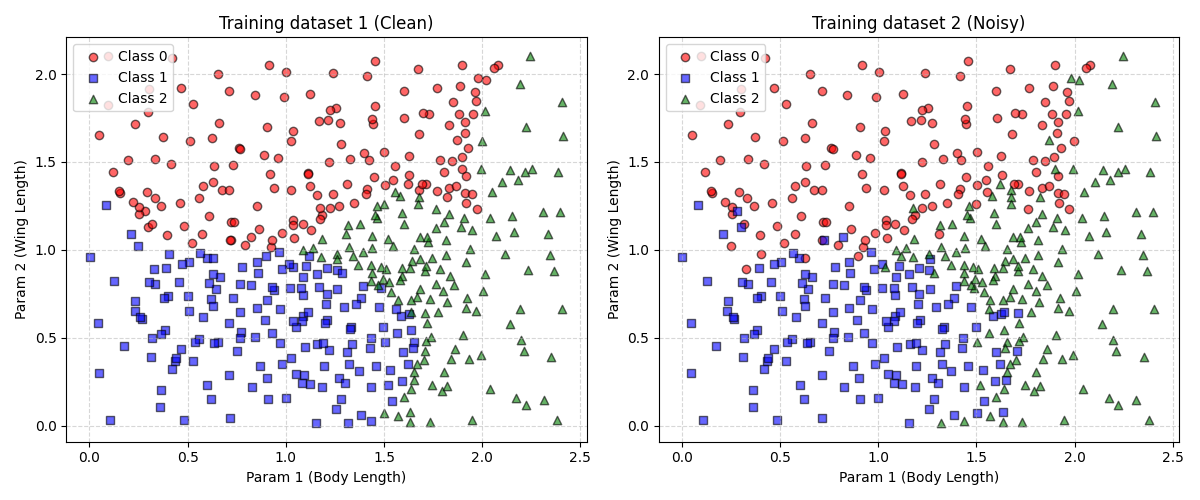
\includegraphics[width=0.9\textwidth]{datavis}
		\caption{昆虫分类训练集数据分布可视化}
		\label{fig:datavis}
	\end{figure}
	
		\begin{figure}[htbp]
		\centering
		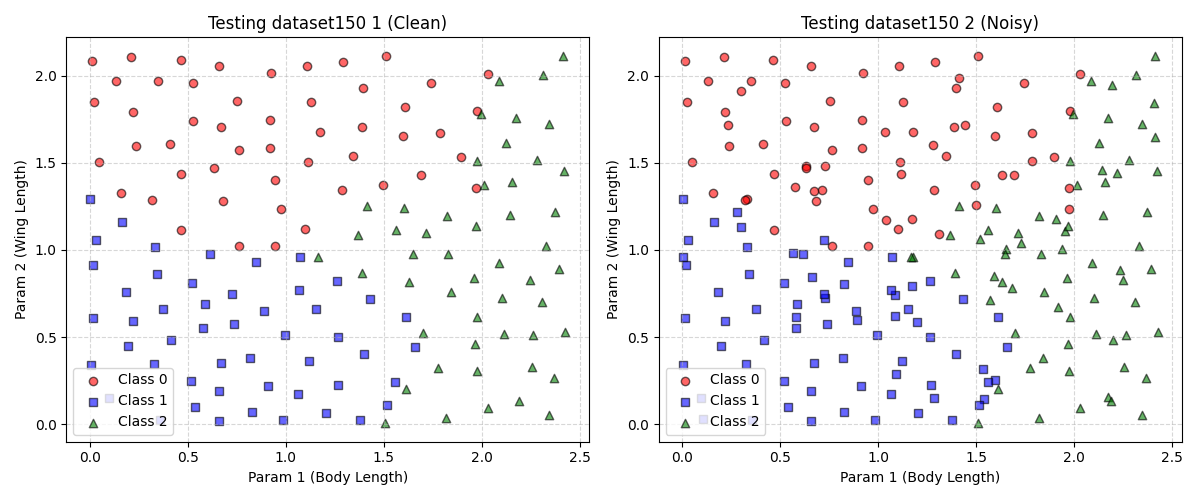
\includegraphics[width=0.9\textwidth]{datavis2}
		\caption{昆虫分类测试集数据分布可视化}
		\label{fig:datavis2}
	\end{figure}
	
\section{实验设计与模型设计}

\subsection{数据特性分析与预处理}
本实验涉及两个维度高度相关的特征：体长（Param 1）与翼长（Param 2）。通过对数据集的可视化（见图\ref{fig:datavis}），可以观察到三个类别在特征空间中呈现出非线性分布。

数据集 2 与数据集 1 的本质区别在于类别边界处的“相互渗透”。这种噪声并非单纯的离群点，而可以视作测量误差导致的统计扰动，这对模型的稳健性提出了更高要求。

\subsection{神经网络算法实现}

\subsubsection{监督学习下的多分类建模}
我们将该任务建模为一个标准的正规{监督学习}下的{多分类}问题。给定标注数据集 $\mathcal{D} = \{(\mathbf{x}_i, y_i)\}_{i=1}^N$，其中 $\mathbf{x}_i$ 表示输入特征向量，$y_i \in \{0, 1, 2\}$ 为离散的类别标签。神经网络的目标是通过学习训练数据，构建一个映射函数 $f: \mathbf{x} \to \hat{\mathbf{y}}$，使预测的概率分布 $\hat{\mathbf{y}}$ 尽可能逼近真实的标签分布。

\subsubsection{神经网络基本原理}
神经网络通过多层非线性变换实现特征的逐层提取与抽象：
\begin{itemize}
	\item \textbf{神经元计算}：每一层 $l$ 的神经元接收前一层的输出 $\mathbf{a}^{(l-1)}$，通过线性加权与偏置叠加后，施加非线性激活函数 $\sigma$（如 ReLU）：
	$$ \mathbf{a}^{(l)} = \sigma(\mathbf{W}^{(l)} \mathbf{a}^{(l-1)} + \mathbf{b}^{(l)}) $$
	\item \textbf{Softmax 输出}：在输出层，采用 Softmax 函数对原始得分进行归一化，生成样本 $i$ 属于类别 $c$ 的预测概率 $\hat{y}_{ic}$，满足 $\sum_c \hat{y}_{ic} = 1$。
\end{itemize}

\subsubsection{训练神经网络的基本流程}
神经网络的训练过程本质上是参数 $\theta = \{\mathbf{W}, \mathbf{b}\}$ 的优化过程，包含以下五个核心步骤：
\begin{enumerate}
	\item \textbf{参数初始化}：对模型权重进行随机初始化（如 Xavier 初始化），以打破对称性。
	\item \textbf{前向传播}：将特征输入网络，逐层计算激活值，最终得到预测值 $\hat{y}$。
	\item \textbf{计算损失}：利用损失函数衡量预测值与真实标签之间的偏差。
	\item \textbf{反向传播}：基于链式法则计算损失函数对各层参数的梯度 $\nabla_{\theta} \mathcal{L}$。
\item \textbf{参数更新}：选用 \textbf{Adam 优化器}。该算法通过计算梯度的一阶矩估计 $m_t$（动量）和二阶矩估计 $v_t$（自适应学习率因子）来动态调整每个参数的更新步长：
\begin{align*}
	m_t &= \beta_1 m_{t-1} + (1 - \beta_1) g_t \\
	v_t &= \beta_2 v_{t-1} + (1 - \beta_2) g_t^2 \\
	\theta_{t+1} &= \theta_t - \frac{\eta}{\sqrt{\hat{v}_t} + \epsilon} \hat{m}_t
\end{align*}
其中 $g_t$ 为当前梯度，$\hat{m}_t$ 和 $\hat{v}_t$ 为经偏差修正后的矩估计，$\eta$ 为学习率。
\end{enumerate}

\subsubsection{损失函数：交叉熵}
为了度量预测概率分布与真实分布的距离，引入\textbf{交叉熵损失函数（Cross-Entropy Loss）}。其数学表达式为：
$$ \mathcal{L}(\theta) = -\frac{1}{N} \sum_{i=1}^{N} \sum_{c=0}^{2} y_{ic} \log(\hat{y}_{ic}) $$
其中，$y_{ic}$ 是真实标签的 One-hot 编码。最小化该函数等价于最大化模型对正确类别的预测似然度。

\subsubsection{评价指标的数学定义}
为了严谨评估模型性能，定义训练误差与测试误差。设 $I(\cdot)$ 为指示函数：
\begin{itemize}
	\item \textbf{训练误差}：在训练集 $\mathcal{D}_{train}$ 上的平均分类错误率：
	$$ E_{train} = \frac{1}{N_{train}} \sum_{i \in \mathcal{D}_{train}} I\left(\text{argmax}_c(\hat{y}_{ic}) \neq y_i\right) $$
	\item \textbf{测试误差}：在独立的测试集 $\mathcal{D}_{test}$ 上的平均分类错误率：
	$$ E_{test} = \frac{1}{N_{test}} \sum_{i \in \mathcal{D}_{test}} I\left(\text{argmax}_c(\hat{y}_{ic}) \neq y_i\right) $$
\end{itemize}

\subsubsection{评价指标的实际意义}
\begin{itemize}
	\item \textbf{拟合能力}：训练误差反映了模型在已知数据上的学习效果。过高的训练误差通常意味着模型容量不足（欠拟合）。
	\item \textbf{泛化能力}：测试误差衡量了模型对未见样本的预测能力。通过观察训练误差与测试误差的差值，可以有效识别\textbf{过拟合}现象：即模型过度拟合了训练集的噪声，导致其在实际应用（测试集）中表现不佳。
\end{itemize}

\subsection{对比实验设计逻辑}
为了深入探讨神经网络在昆虫分类任务中的表现机理，本实验设计了以下三个维度的对比实验：

\subsubsection{模型复杂度}
旨在探究模型容量与任务复杂度的匹配关系。
\begin{itemize}
	\item \textbf{模型 A (Baseline)}：32-16 隐藏层结构。作为本实验的基准架构。
	\item \textbf{模型 B (Minimal)}：线性感知机，不设隐藏层。用以验证分类任务是否具备线性可分性。
	\item \textbf{模型 C (Complex)}：3 层隐藏层，每层 64 神经元。
	\item \textbf{模型 D (Overfitting)}：4 层隐藏层，每层 64 神经元。观察在样本量受限或者样本存在噪声时，过大的假设空间是否会导致模型过度拟合噪声。
\end{itemize}

\subsubsection{激活函数对比：决策边界的几何连续性}
探究非线性映射的刻画能力。
\begin{itemize}
	\item \textbf{ReLU 方案}：$ \sigma(z) = \max(0, z) $。其生成的决策边界本质上是多个超平面的分段线性组合，训练效率高，但边界可能存在尖锐转折。
	
	\item \textbf{Sigmoid 方案}：$ \sigma(z) = \frac{1}{1 + e^{-z}} $。该函数将输出映射至 $ (0, 1) $ 区间。其具备 $ C^\infty $ 连续性，生成的决策边界更为平滑。
	
	\item \textbf{Tanh 方案}：$ \sigma(z) = \frac{e^z - e^{-z}}{e^z + e^{-z}} $。该函数将输出映射至 $ (-1, 1) $ 区间。其具备 $ C^\infty $ 连续性，生成的决策边界更为平滑。
	
	\item \textbf{LeakyReLU 方案}：$ \sigma(z) = \max(\alpha z, z) $。针对 ReLU 存在的“神经元坏死”问题进行了改进，在 $ z < 0 $ 区域保留了一个微小的斜率（本实验取 $ \alpha = 0.1 $），确保在负值区间仍能维持有效的梯度传导，提升了训练的鲁棒性。
	
\end{itemize}

\subsection{决策边界可视化}

本实验中，通过对全域特征空间进行绘图，可以直观展现不同模型在分类上的差异，作为评估模型欠拟合、过拟合的重要依据。

\section{其它分类算法}

\subsection{KNN 算法 (K-Nearest Neighbors)}

KNN是一种基于实例的学习算法，其核心思想是“物以类聚”。在分类阶段，KNN 不进行显式的模型训练，而是通过计算待测样本与训练集样本在特征空间中的距离来实现归类。

\subsubsection{分类逻辑与数学表达}
对于给定测试样本 $\mathbf{x}$，算法首先在训练集中寻找与之欧式距离最近的 $k$ 个邻居，这里距离一般采用欧氏距离。$k$为本算法的超参数，在$k$较小时一般采用$k$为奇数以避免边界处出现两类样本混淆的情况。最终分类结果由这 $k$ 个邻居的类别进行“多数表决”决定：$$\hat{y} = \arg \max_{c} \sum_{\mathbf{x}_i \in N_k(\mathbf{x})} I(y_i = c)$$其中 $I(\cdot)$ 为指示函数，$N_k(\mathbf{x})$ 表示 $\mathbf{x}$ 的 $k$ 个近邻集合。

\subsubsection{算法特性}

\begin{itemize}
	\item \textbf{非参数化}：无需对数据分布做先验假设，能够灵活地捕捉如实验中观察到的“弧形”决策边界。
	
	\item \textbf{对噪声敏感}：在数据集 2 这种存在边界重叠的情况下，较小的 $k$ 值容易导致过拟合，而较大的 $k$ 值则可能导致边界模糊。
\end{itemize}

\subsubsection{决策边界可视化}
在KNN的决策边界可视化中，若一个点有多种结果，则绘制该点时采用所有结果的平均颜色。不过由于选取$k$为奇数，这样的区域一般较小，所以在图上混合色区域往往并不明显。

\subsection{SVM 算法 (Support Vector Machine)}

支持向量机（SVM）的原始目标是寻找一个超平面，使得两类样本之间的几何间隔最大化。针对本实验的三分类及非线性可分任务，SVM 通过核技巧和多分类策略进行扩展。算法要求输入训练数据集  $T=\left\{ \left( \boldsymbol{x}_1,y_1 \right) ,\left( \boldsymbol{x}_2,y_2 \right) ,...,\left( \boldsymbol{x}_N,y_N \right) \right\}$ 其中$\boldsymbol{x}_i\in \mathbb{R}^n , y_i\in \left\{ +1,-1 \right\} ,i=1,2,...,N.$\footnote{3.2.1和3.2.2引用自周志华《机器学习》}

\subsubsection{非线性映射与核技巧动机}
在本研究的昆虫分类任务中，由于不同物种的特征分布在原始低维空间中存在严重的重叠，呈现出明显的非线性分布特征，传统的线性超平面难以实现有效分割。
为此，我们引入 \textbf{RBF 高斯核函数（Radial Basis Function Kernel）}。其核心动机在于：通过一种隐式的非线性映射 $\phi(\cdot)$，将原始特征空间投影到高维甚至无穷维的特征空间，使得在该高维空间中原本线性不可分的样本变得线性可分。

高斯核函数的数学定义为：
$$ K(\mathbf{x}_i, \mathbf{x}_j) = \phi(\mathbf{x}_i)^T \phi(\mathbf{x}_j) = \exp\left(-\gamma \|\mathbf{x}_i - \mathbf{x}_j\|^2\right) $$
该核函数本质上是一种相似度度量：当两样本距离极近时，其核值趋近于 1；反之趋近于 0。通过调节参数 $\gamma$，模型可以灵活地控制局部影响力的范围，从而构建极其平滑且复杂的非线性决策边界。

\subsubsection{带有高斯核的优化目标}
由于核映射 $\phi(\mathbf{x})$ 的具体形式往往难以显式表达，SVM 的优化目标通常从原问题转化为其拉格朗日对偶问题。在该形式下，高斯核函数 $K(\mathbf{x}_i, \mathbf{x}_j)$ 可以直接替代映射后的内积项。

考虑软间隔约束，带有核函数的对偶优化目标定义如下：
\begin{align*}
	\max_{\alpha} \quad & \sum_{i=1}^{N} \alpha_i - \frac{1}{2} \sum_{i=1}^{N} \sum_{j=1}^{N} \alpha_i \alpha_j y_i y_j K(\mathbf{x}_i, \mathbf{x}_j) \\
	\text{s.t.} \quad & \sum_{i=1}^{N} \alpha_i y_i = 0 \\
	& 0 \leq \alpha_i \leq C, \quad i=1, \dots, N
\end{align*}

其中：
\begin{itemize}
	\item $\alpha_i$ 是每个样本对应的拉格朗日乘子。只有 $\alpha_i > 0$ 的样本被称为\textbf{支持向量}，决定了最终的决策边界。
	\item $C$ 为惩罚因子（正则化参数）。较大的 $C$ 倾向于对训练集实现零误差分类（易导致过拟合）；较小的 $C$ 则允许部分样本位于间隔带内或被误分，从而通过权衡偏置与方差，增强模型在测试集上的泛化能力。
\end{itemize}

最终的非线性决策函数表示为：
$$ f(\mathbf{x}) = \text{sign} \left( \sum_{i \in SV} \alpha_i y_i K(\mathbf{x}_i, \mathbf{x}) + b \right) $$

\subsubsection{多分类策略}
针对多分类任务，通常采用 \textbf{OvO (One-vs-One)} 策略，对每两个类都设置一个分类器，最终“每个分类器进行投票”，“得票”最多者获胜。由于平票对应是空间中一条线，所以概率认为是0。

\subsection{评价指标的数学定义与实际意义}
为了量化评估 SVM 在多分类任务下的性能，定义如下指标：
\begin{itemize}
	\item \textbf{测试误差}：
	$$ E_{test} = \frac{1}{N_{test}} \sum_{i=1}^{N_{test}} I\left( f(\mathbf{x}_i) \neq y_i \right) $$
	该指标反映了模型在处理未见过样本时的稳健性。
	\item \textbf{实际意义}：在昆虫识别实际应用中，较低的测试误差意味着模型能够从复杂的自然环境中准确辨识物种。通过观察训练误差与测试误差的差值，可以指导我们调整 $C$ 与 $\gamma$，以避免模型仅是“死记硬背”了训练数据的噪声。
\end{itemize}

\subsection{额外优化细节}
\begin{enumerate}
	\item 由于两个轴单位长度并不相等，所以使用使用 \texttt{StandardScaler} 将数据缩放到均值为 0、方差为 1 的区间。
	
	\item 由于两个超参数调节较为复杂，所以直接采用网格搜索的方式，对$C \in [0.1, 1, 10, 100, 1000, 10000]$，$ \gamma \in [0.001, 0.01, 0.1, 1, 10]$ 进行网格式搜索，最终只输出最优参数的结果并绘图。
\end{enumerate}

	
\section{结果}

\subsection{模型容量对结果的影响}

本节通过构建四种不同复杂度的模型Model A（基准）、Model B（线性）、Model C（复杂）及 Model D（过拟合），探讨假设空间容量对昆虫分类任务的影响。\textbf{由于观察到模型较大时训练具有较强的不确定性，为了更有说服力的说明各个模型的效果，我们进行了10次实验对结果取平均值和标准差并截取两次比较有代表性的实验结果如下}。

\begin{table}[htbp]
	\centering
	\caption{不同容量模型在两类数据集下的分类表现（10次实验统计）}
	\label{tab:performance_stat}
	\small
	\begin{tabular}{lccc}
		\toprule
		模型名称 & 训练集准确率 & 测试集 (Top 60) & 测试集 (Last 150) \\
		\midrule
		\multicolumn{4}{l}{\textbf{数据集 1 (无噪 - Clean)}} \\
		Model A (Baseline) & 99.29\% $\pm$ 0.42\% & 99.17\% $\pm$ 1.34\% & 98.67\% $\pm$ 0.94\% \\
		Model B (Linear)   & 88.29\% $\pm$ 0.22\% & 87.33\% $\pm$ 0.82\% & 89.00\% $\pm$ 0.54\% \\
		Model C (Complex)  & \textbf{99.33\% $\pm$ 1.15\%} & \textbf{99.67\% $\pm$ 0.67\%} & \textbf{98.93\% $\pm$ 1.40\%} \\
		Model D (Overfit)  & 98.56\% $\pm$ 2.51\% & 98.67\% $\pm$ 2.08\% & 98.07\% $\pm$ 2.88\% \\
		\midrule
		\multicolumn{4}{l}{\textbf{数据集 2 (含噪 - Noisy)}} \\
		Model A (Baseline) & 90.71\% $\pm$ 0.96\% & 89.17\% $\pm$ 2.50\% & \textbf{95.47\% $\pm$ 0.98\%} \\
		Model B (Linear)   & 85.38\% $\pm$ 0.36\% & 87.33\% $\pm$ 0.82\% & 89.67\% $\pm$ 0.80\% \\
		Model C (Complex)  & 92.93\% $\pm$ 1.03\% & 91.83\% $\pm$ 2.03\% & 95.33\% $\pm$ 0.94\% \\
		Model D (Overfit)  & \textbf{94.00\% $\pm$ 1.13\%} & \textbf{93.17\% $\pm$ 3.61\%} & 94.80\% $\pm$ 0.58\% \\
		\bottomrule
	\end{tabular}
\end{table}

\begin{figure}[htbp]
	\centering
	\begin{minipage}{0.48\textwidth}
		\centering
		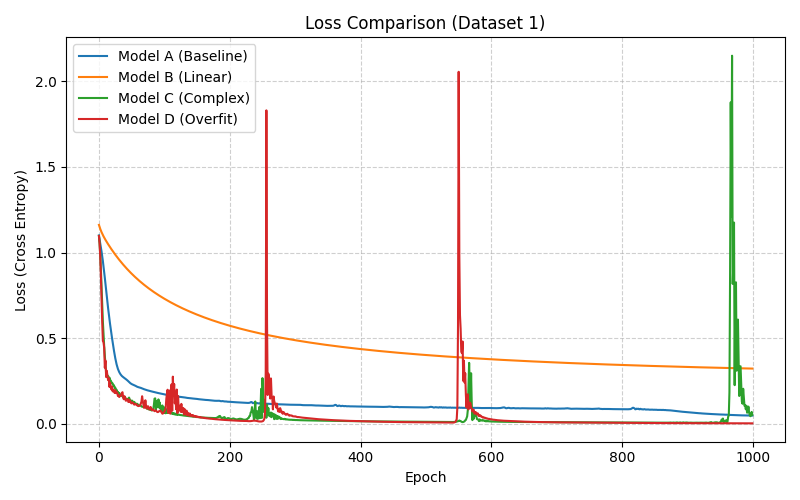
\includegraphics[width=\textwidth]{loss cmp 1}
		\caption{数据集 1 训练损失对比（第一次）}
		\label{fig:loss_1}
	\end{minipage}
	\hfill
	\begin{minipage}{0.48\textwidth}
		\centering
		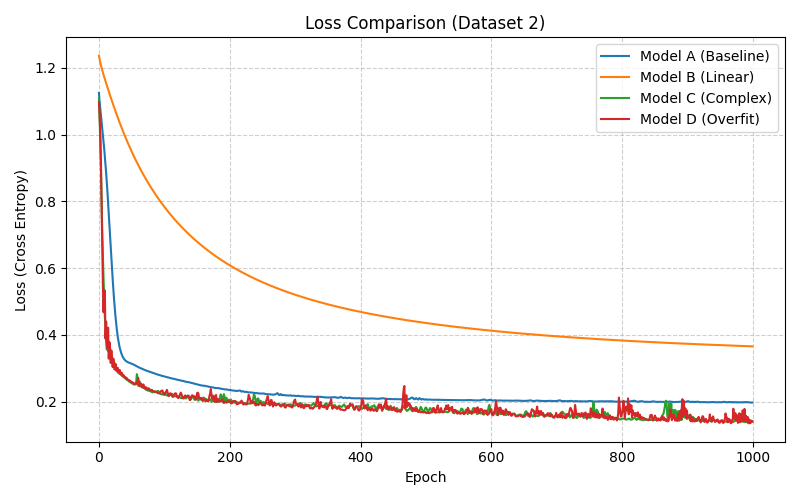
\includegraphics[width=\textwidth]{loss cmp 2}
		\caption{数据集 2 训练损失对比（第一次）}
		\label{fig:loss_2}
	\end{minipage}
	\label{fig:loss_compare}
\end{figure}


\begin{figure}[htbp]
	\centering
	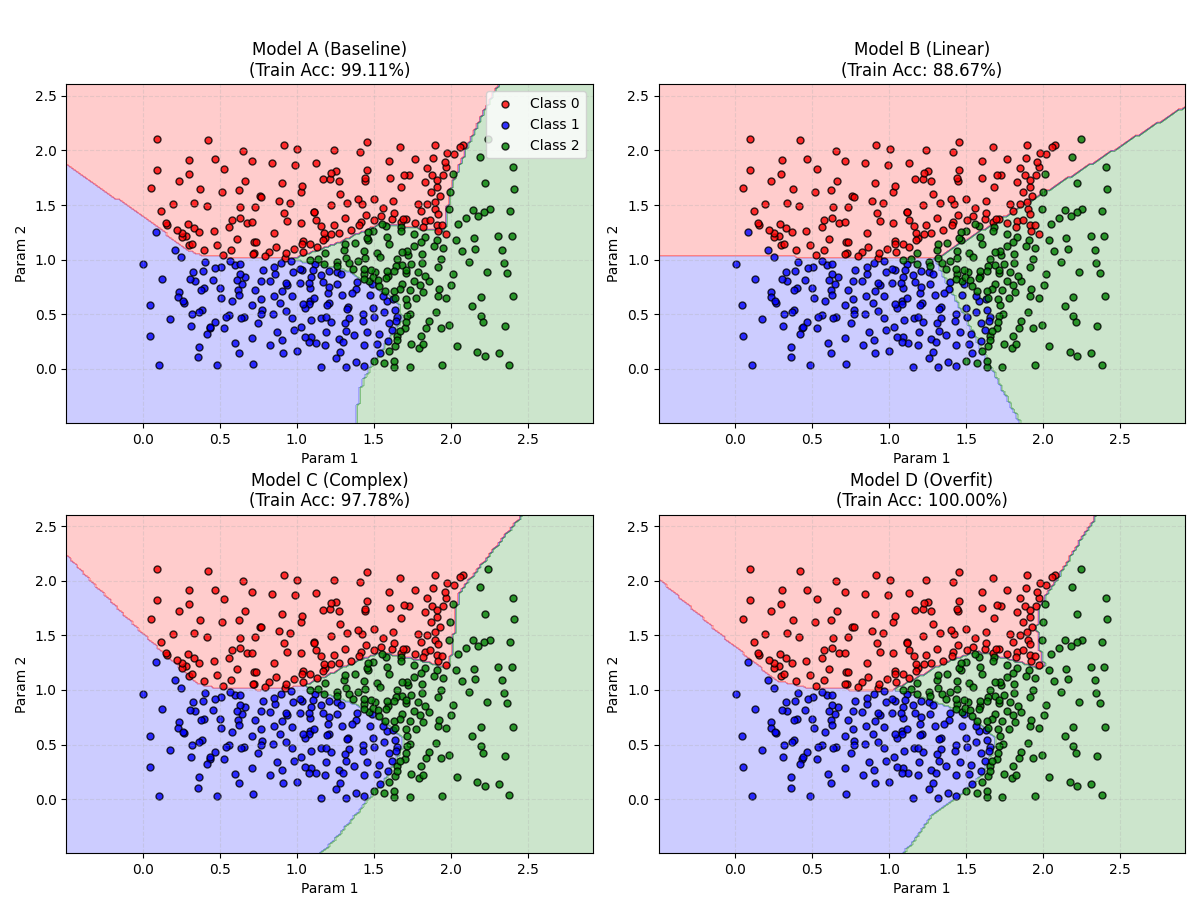
\includegraphics[width=0.9\textwidth]{1 train acc}
	\caption{第一次实验：数据集 1（不含噪）下不同容量模型的决策边界和训练集对比}
	\label{fig:1_train_acc}
\end{figure}

\begin{figure}[htbp]
	\centering
	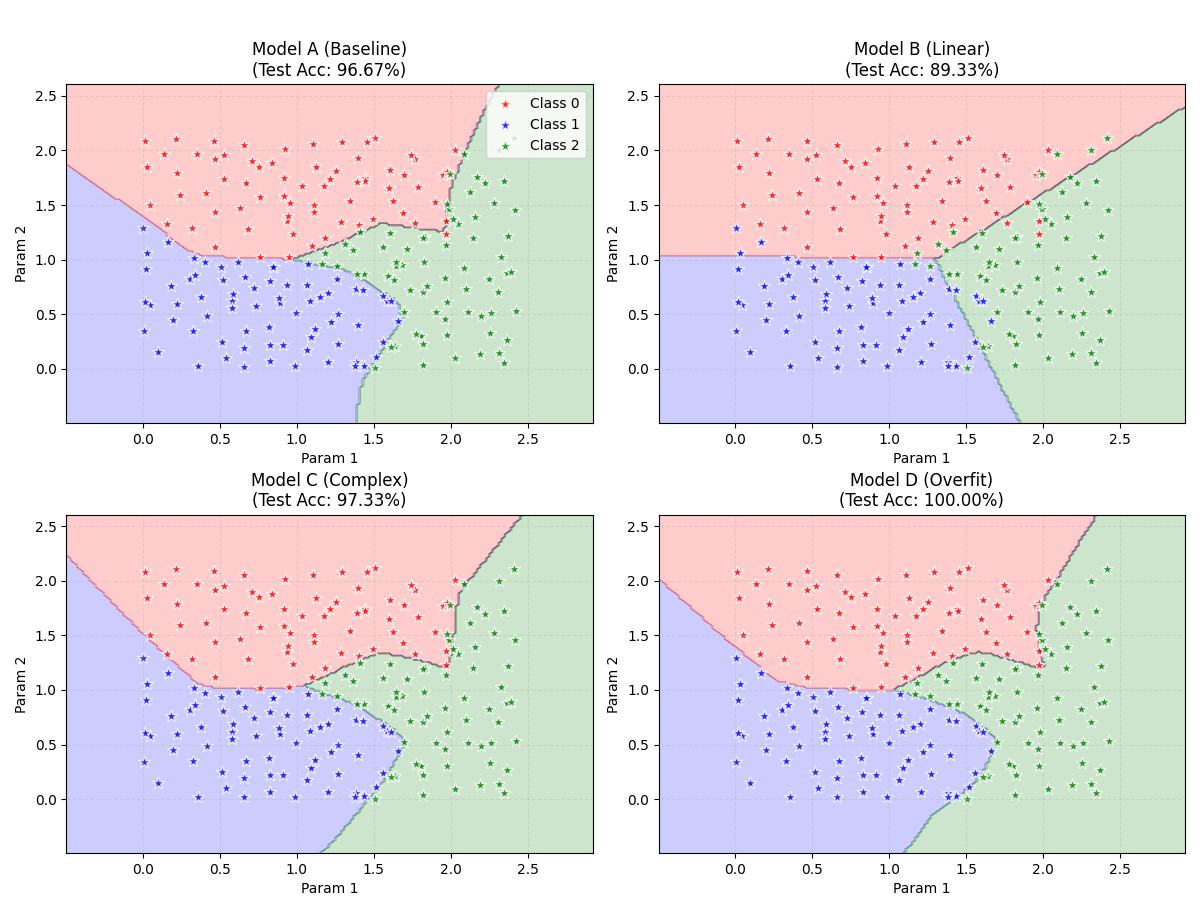
\includegraphics[width=0.9\textwidth]{1 test acc}
	\caption{第一次试验：数据集 1（不含噪）下不同容量模型的决策边界和测试集对比}
	\label{fig:1_test_acc}
\end{figure}

\begin{figure}[htbp]
	\centering
	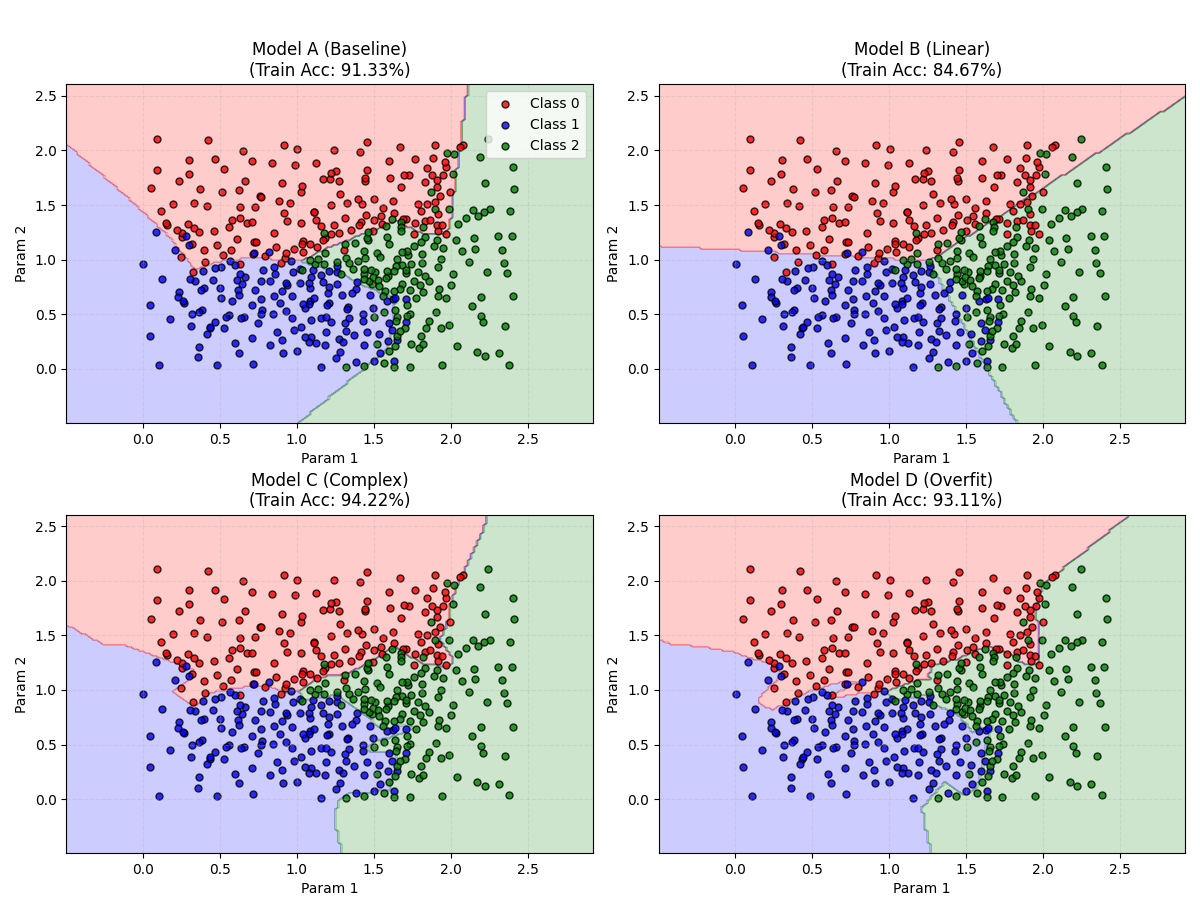
\includegraphics[width=0.9\textwidth]{2 train acc}
	\caption{第一次实验：数据集 2（含噪）下不同容量模型的决策边界和训练集对比}
	\label{fig:2_train_acc}
\end{figure}

\begin{figure}[htbp]
	\centering
	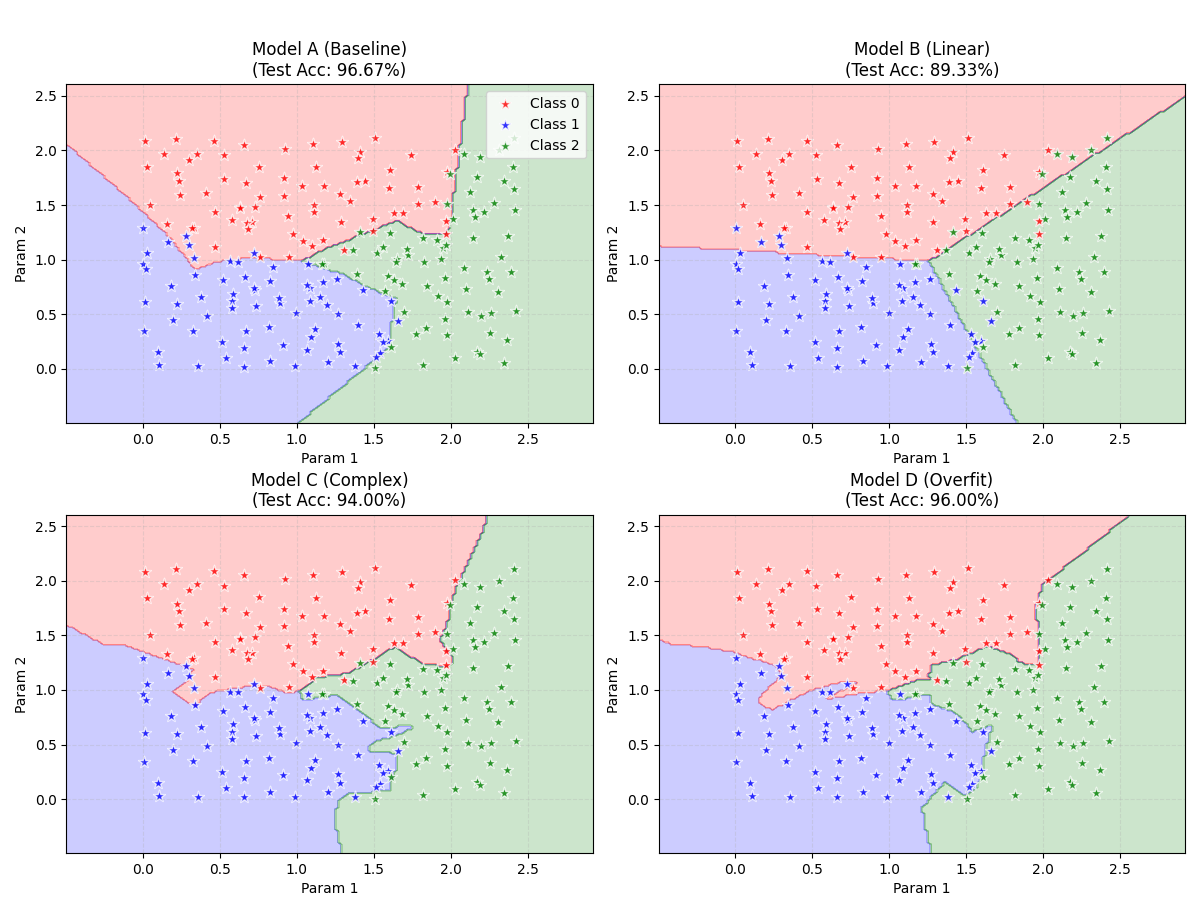
\includegraphics[width=0.9\textwidth]{2 test acc}
	\caption{第一次试验：数据集 2（含噪）下不同容量模型的决策边界和测试集对比}
	\label{fig:2_test_acc}
\end{figure}

\begin{figure}[htbp]
	\centering
	\begin{minipage}{0.48\textwidth}
		\centering
		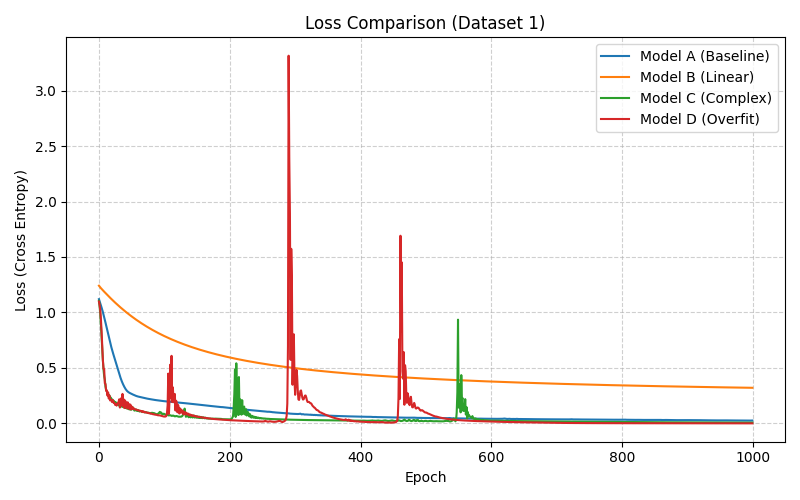
\includegraphics[width=\textwidth]{loss cmp 1'}
		\caption{数据集 1 训练损失对比（第二次）}
		\label{fig:loss_1'}
	\end{minipage}
	\hfill
	\begin{minipage}{0.48\textwidth}
		\centering
		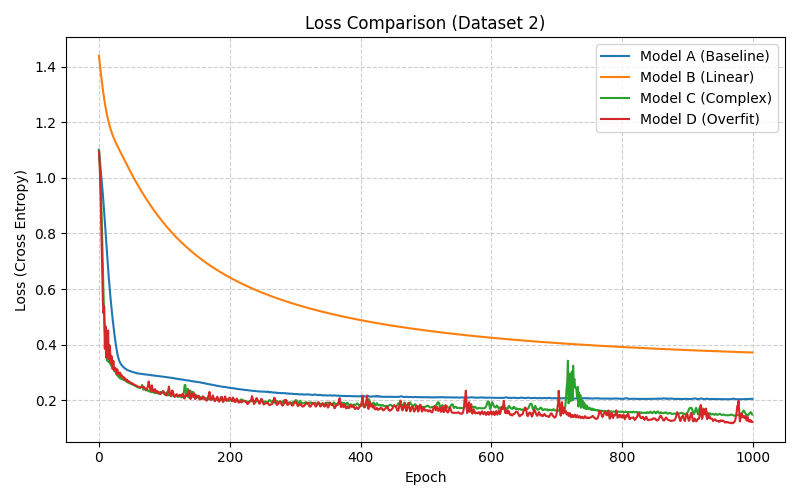
\includegraphics[width=\textwidth]{loss cmp 2'}
		\caption{数据集 2 训练损失对比（第二次）}
		\label{fig:loss_2'}
	\end{minipage}
	\label{fig:loss_compare'}
\end{figure}

\begin{figure}[htbp]
	\centering
	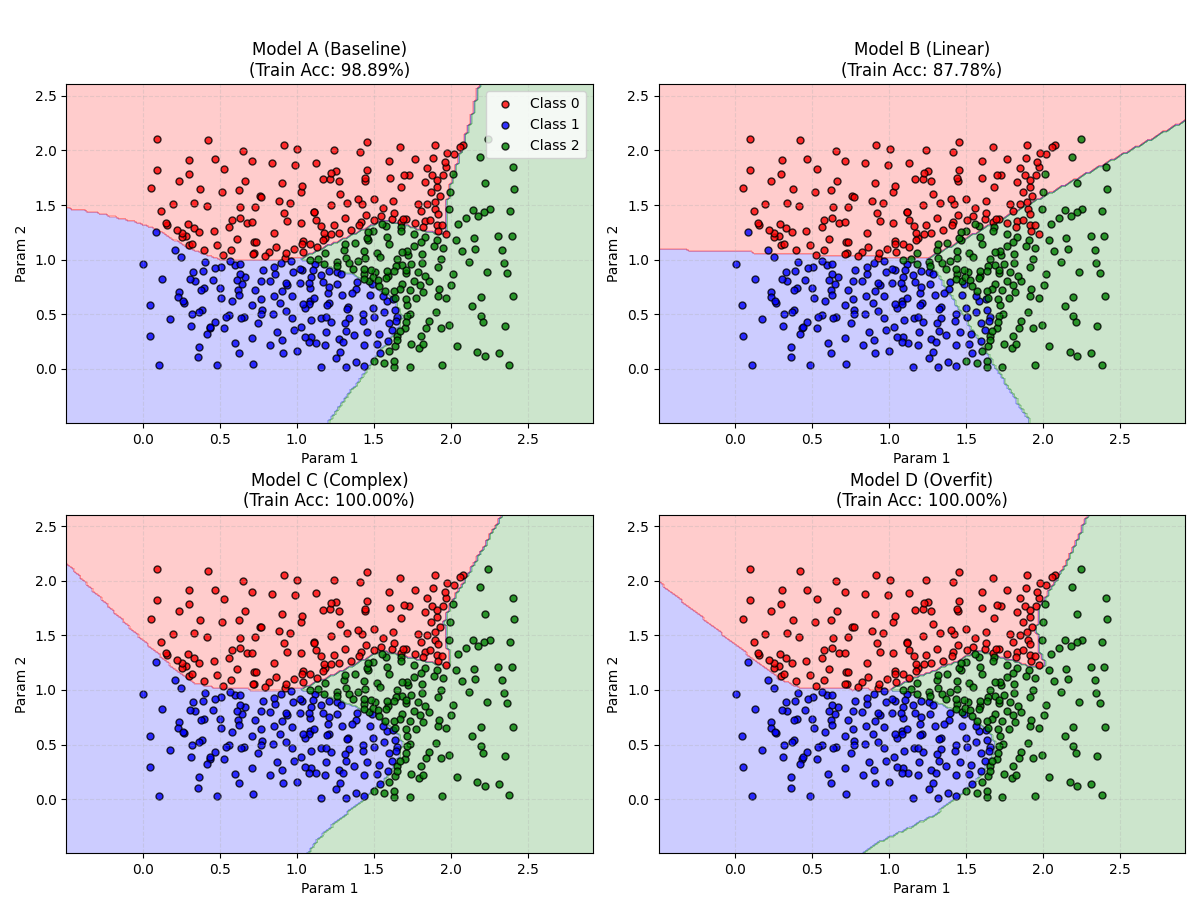
\includegraphics[width=0.9\textwidth]{1 train acc'}
	\caption{第二次实验：数据集 1（不含噪）下不同容量模型的决策边界和训练集对比}
	\label{fig:1_train_acc'}
\end{figure}

\begin{figure}[htbp]
	\centering
	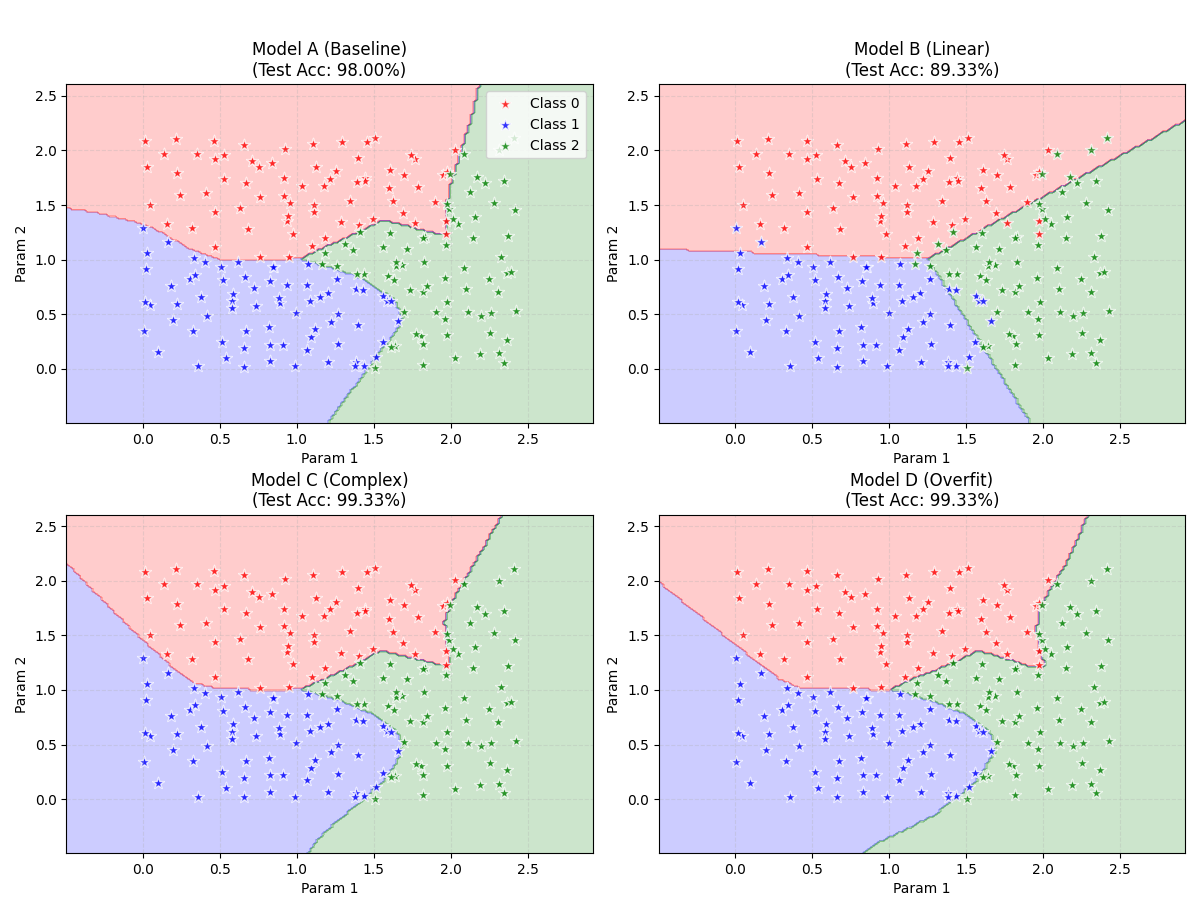
\includegraphics[width=0.9\textwidth]{1 test acc'}
	\caption{第二次试验：数据集 1（不含噪）下不同容量模型的决策边界和测试集对比}
	\label{fig:1_test_acc'}
\end{figure}

\begin{figure}[htbp]
	\centering
	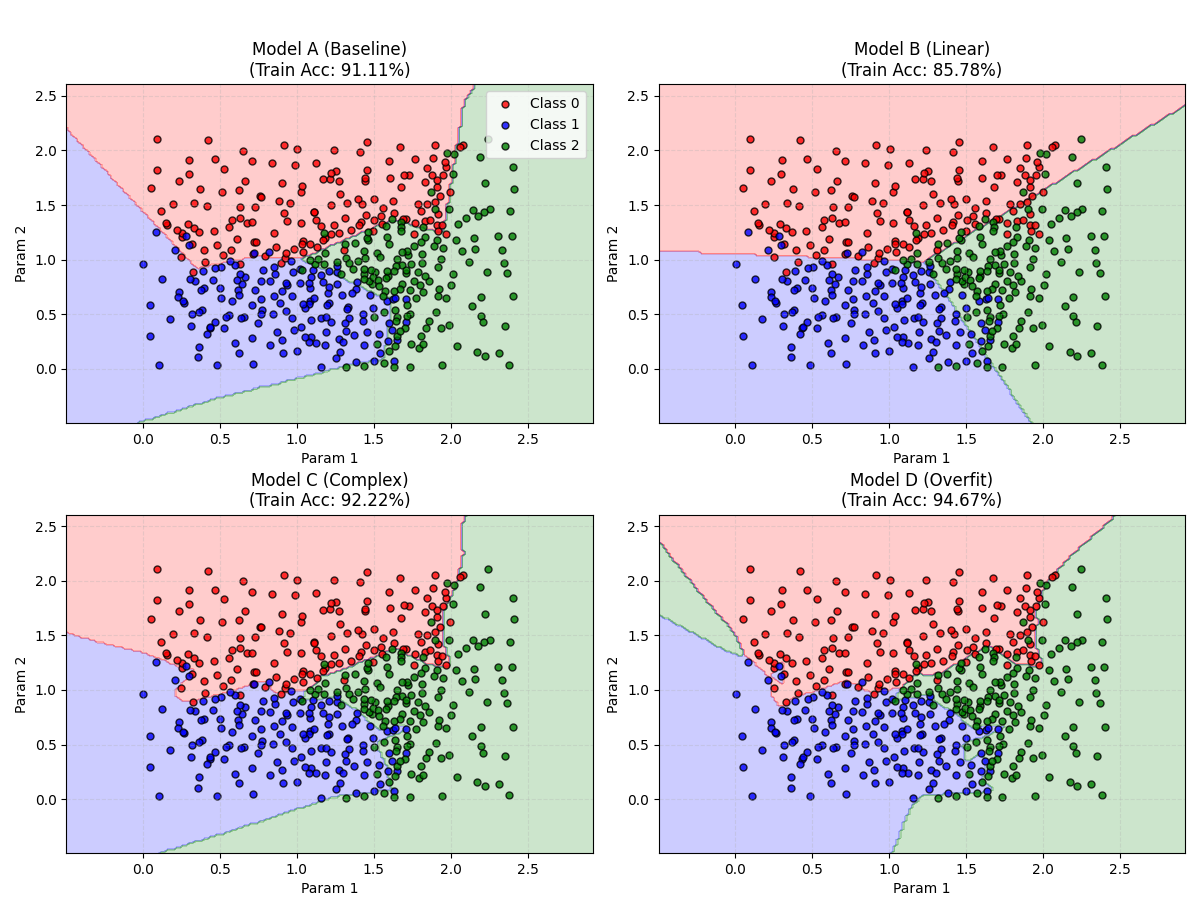
\includegraphics[width=0.9\textwidth]{2 train acc'}
	\caption{第二次实验：数据集 2（含噪）下不同容量模型的决策边界和训练集对比}
	\label{fig:2_train_acc'}
\end{figure}

\begin{figure}[htbp]
	\centering
	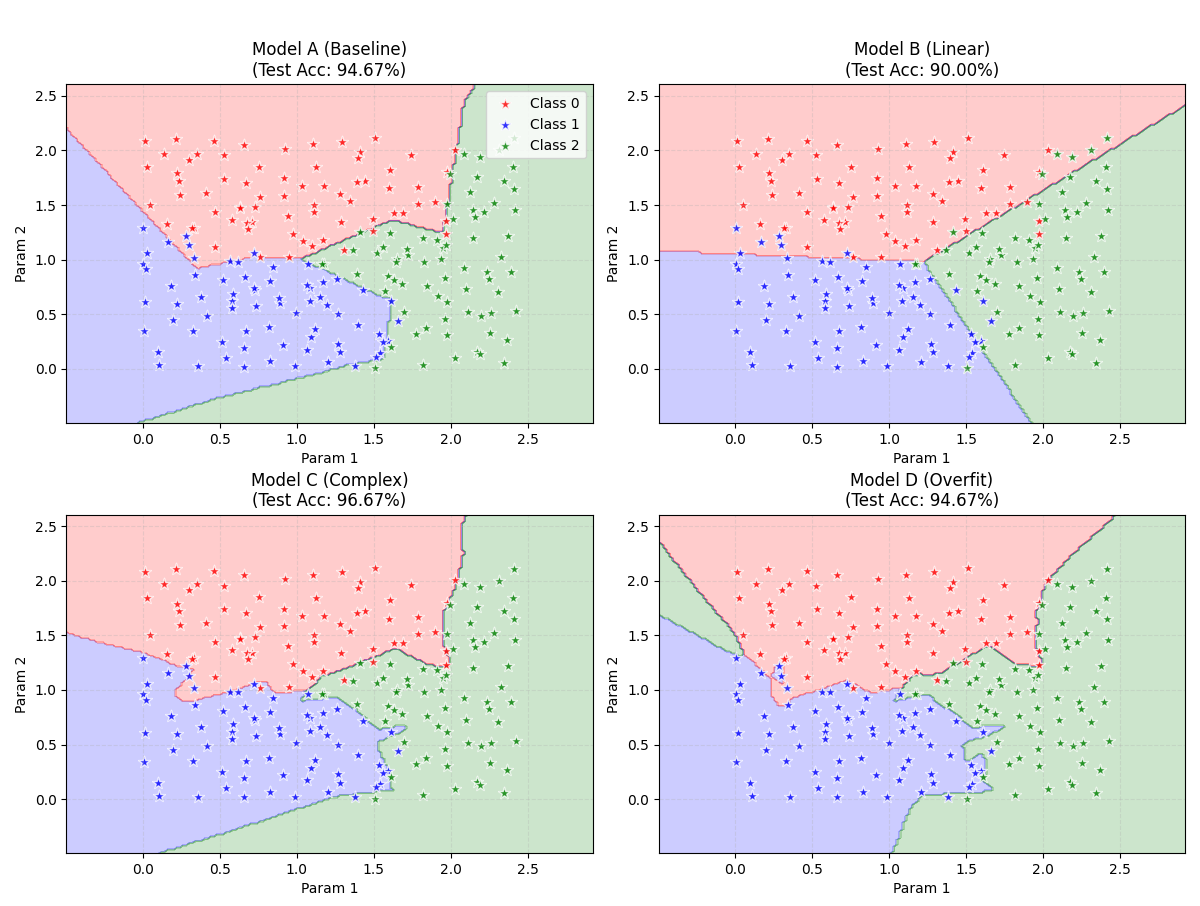
\includegraphics[width=0.9\textwidth]{2 test acc'}
	\caption{第二次试验：数据集 2（含噪）下不同容量模型的决策边界和测试集对比}
	\label{fig:2_test_acc'}
\end{figure}


\subsubsection{分类表现与泛化性能分析}
根据测试集（后150个新数据）的准确率统计，我们可以得出以下结论：

\begin{itemize}
	\item \textbf{线性模型的局限性}：Model B 由于缺乏隐藏层，其决策边界仅为线性超平面。虽然其训练稳健，但在处理具有非线性特征的昆虫数据时存在明显的欠拟合，最高准确率仅为 90.00\%。
	\item \textbf{复杂模型的不确定性}：在理想数据集 1 中，随着网络深度的增加，模型的拟合能力显著增强。Model C,D 凭借极大的参数空间，在无噪环境下可以达到 99.33\% 和 100.00\% 的完美分类。但是由于过大模型训练的不确定性，导致其表现不稳定，相对于基准B模型表现时而更好时而更坏。
	\item \textbf{高容量模型的双刃剑效应}：例如 Model D 在数据集 1 上表现完美，但在数据集 2 中准确率反而下降严重，甚至不如基准模型B，观察到图中模型D的决策区域出现过多锯齿状结构和左侧的异常绿色区域，这表明模型开始尝试拟合测量误差（噪声），从而产生了过拟合现象。
\end{itemize}

\subsubsection{训练稳定性与收敛特性}
观察损失曲线图可以发现一个显著的数值现象：

\begin{enumerate}
	\item \textbf{数值不稳定性}：在数据集 1 的训练过程中，高容量模型（Model C 和 Model D）在 某些Epoch上出现了剧烈的损失值瞬时激增）。
	\item \textbf{噪声的平滑作用}：有趣的是，在数据集 2 中，由于数据本身存在的随机噪声起到了一定的“天然正则化”作用，使得各模型的 Loss 曲线虽然收敛值较高，但过程反而比数据集 1 更加平稳，未出现剧烈抖动。
\end{enumerate}

\subsubsection{实验小结}
在无噪声的数据集下，Model C (Complex) 的表现最好，不过相对于Model A (Baseline) 差别不算大，并且标准差更大，是复杂模型训练不稳定所致。在有噪音的数据集下，Model A (Baseline) 表现最好。

模型容量必须与问题的复杂程度及噪声水平相匹配。例如 Model D 虽然在理想条件下具备极高的拟合上限，但其过强的假设空间捕捉能力和训练时的不稳定性使其表现出较弱的鲁棒性。

\subsection{激活函数对实验结果的影响}在本组实验中，我们固定了神经网络的拓扑结构（隐藏层为 $[32, 16]$的Baseline Model），仅改变隐藏层所使用的非线性激活函数，并对每种配置进行了 10 次独立重复实验以消除初始化随机性的影响。实验分别在干净数据集（Dataset 1）和含噪声数据集（Dataset 2）上进行。

\subsubsection{实验数据汇总}

下表展示了四种常见激活函数（ReLU, Sigmoid, Tanh, LeakyReLU）在两个数据集上的平均准确率及标准差，并截取了一次具有代表性的实验的详细实验数据。

% --- 表格 1 ---
\begin{table}[htbp]
	\centering
	\caption{不同激活函数在 Dataset 1（Clean）上的表现对比}
	\begin{tabular}{lccc}
		\hline
		\textbf{激活函数} & \textbf{训练集准确率} & \textbf{测试集 60 准确率} & \textbf{测试集 150 准确率} \\ \hline
		ReLU      & 99.27\% $\pm$ 0.60\% & 98.83\% $\pm$ 1.30\% & 99.07\% $\pm$ 0.61\% \\
		Sigmoid   & 99.62\% $\pm$ 0.14\% & 99.83\% $\pm$ 0.50\% & 99.60\% $\pm$ 0.61\% \\
		Tanh      & \textbf{99.87\% $\pm$ 0.11\%} & \textbf{100.00\% $\pm$ 0.00\%} & \textbf{99.87\% $\pm$ 0.27\%} \\
		LeakyReLU & 99.38\% $\pm$ 0.58\% & 99.00\% $\pm$ 1.11\% & 98.53\% $\pm$ 1.33\% \\ \hline
	\end{tabular}
\end{table}

% --- 表格 2 ---
\begin{table}[htbp]
	\centering
	\caption{不同激活函数在 Dataset 2（Noisy）上的表现对比}
	\begin{tabular}{lccc}
		\hline
		\textbf{激活函数} & \textbf{训练集准确率} & \textbf{测试集 60 准确率} & \textbf{测试集 150 准确率} \\ \hline
		ReLU      & 90.96\% $\pm$ 0.60\% & 88.83\% $\pm$ 0.76\% & \textbf{95.93\% $\pm$ 0.70\%} \\
		Sigmoid   & 90.98\% $\pm$ 0.37\% & 90.00\% $\pm$ 0.75\% & 95.33\% $\pm$ 0.79\% \\
		Tanh      & \textbf{93.58\% $\pm$ 0.86\%} & \textbf{92.67\% $\pm$ 2.00\%} & 95.33\% $\pm$ 1.07\% \\
		LeakyReLU & 91.02\% $\pm$ 0.91\% & 89.33\% $\pm$ 1.11\% & 95.60\% $\pm$ 1.04\% \\ \hline
	\end{tabular}
\end{table}

\begin{figure}[htbp]
	\centering
	\begin{minipage}{0.48\textwidth}
		\centering
		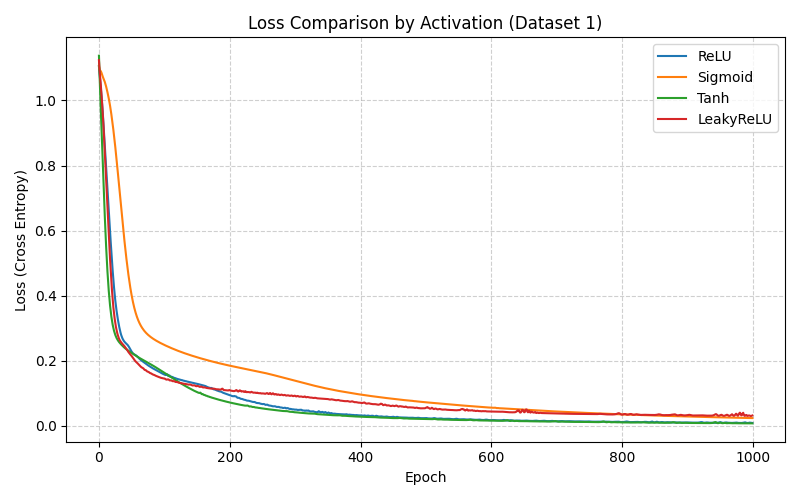
\includegraphics[width=\textwidth]{losscmp1}
		\caption{数据集 1 训练损失对比}
		\label{fig:loss_1act}
	\end{minipage}
	\hfill
	\begin{minipage}{0.48\textwidth}
		\centering
		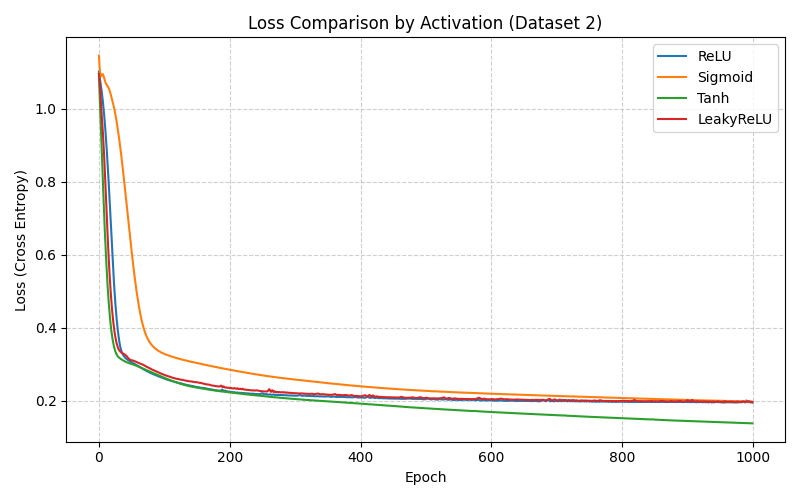
\includegraphics[width=\textwidth]{losscmp2}
		\caption{数据集 2 训练损失对比）}
		\label{fig:loss_2act}
	\end{minipage}
	\label{fig:loss_compare_act}
\end{figure}

\fig{act 1 train acc}{0.9}{数据集1（不含噪）不同激活函数对应的决策边界和训练集对比}

\fig{act 1 test acc}{0.9}{数据集1（不含噪）不同激活函数对应的决策边界和测试集对比}

\fig{act 2 train acc}{0.9}{数据集2（含噪）不同激活函数对应的决策边界和训练集对比}

\fig{act 2 test acc}{0.9}{数据集2（含噪）不同激活函数对应的决策边界和测试对比}

\subsubsection{实验结果分析与讨论}通过对上述实验数据的对比分析，可以得出以下结论：

\begin{enumerate}
	
	\item \textbf{Tanh 激活函数的稳定性：}在两个数据集上，Tanh 函数均表现出了最优的平均准确率，尤其是在 Dataset 1 中达到了接近 100\%的表现且标准差极小。
	
	\item \textbf{饱和区激活函数在浅层网络中的优势：}
	在处理低维特征（本实验为 2 维昆虫特征）且网络层数较浅时，Sigmoid 和 Tanh 等饱和型激活函数反而表现优于 ReLU。这可能是因为饱和函数提供的平滑非线性映射能够生成更“平滑”的决策边界，在特征区分度较高时（Dataset 1），能有效避免 ReLU 可能出现的过度折线化边界，从而获得极高的测试精度。
	
	\item \textbf{噪声环境下的鲁棒性：}
	在含噪声的 Dataset 2 中，所有模型的准确率均有所下降。此时 Tanh 依然保持了最高的训练精度（93.58\%），说明其对于复杂分布的拟合能力较强。观察决策边界可以发现其展现出了一定程度的过拟合。导致训练误差更高的 ReLU 类函数（包括 LeakyReLU）在测试集 150 上的表现比Tanh更佳，这体现了 ReLU 系列函数在处理较大规模或较复杂数据分布时更好的泛化潜力。
	
	\item \textbf{LeakyReLU 与 ReLU 的差异：}
	LeakyReLU 在训练集准确率上优于 ReLU。这是因为 LeakyReLU 在 $x < 0$ 区域保留了一个很小的梯度，解决了 ReLU 可能出现的“神经元坏死”问题。但是其在测试集上误差高于 ReLU，说明其泛化能力较差。
\end{enumerate}\subsubsection{小结}综合来看，针对本实验的昆虫分类任务，\textbf{Tanh 函数}和 \textbf{ReLU函数} 是最优选择。前者拟合性能最强，后者泛化能力最强。在训练集没有噪声的情况下，Tanh函数占优。在训练集有噪声的情况下 ReLU函数占优。

\subsection{KNN实验结果}

\subsubsection{实验数据}

\begin{table}[htbp]
	\centering
	\caption{KNN 算法在不同数据集下的性能对比}
	\label{tab:knn_results}
	\begin{tabular}{lcccc}
		\toprule
		\textbf{数据集类型} & \textbf{KNN 模型 (K)} & \textbf{训练集准确率} & \textbf{测试集 (60)} & \textbf{测试集 (150)} \\
		\midrule
		\multirow{4}{*}{Dataset 1 (Clean)} 
		& KNN ($k=1$) & 100.00\% & 100.00\% & \textbf{98.00\%} \\
		& KNN ($k=3$) & 97.56\%  & 98.33\%  & 95.33\% \\
		& KNN ($k=5$) & 96.00\%  & 96.67\%  & 95.33\% \\
		& KNN ($k=15$)& 95.78\%  & 96.67\%  & 92.00\% \\
		\midrule
		\multirow{4}{*}{Dataset 2 (Noisy)} 
		& KNN ($k=1$) & 100.00\% & 100.00\% & \textbf{95.33\%} \\
		& KNN ($k=3$) & 92.22\%  & 90.00\%  & 92.67\% \\
		& KNN ($k=5$) & 90.44\%  & 90.00\%  & 92.00\% \\
		& KNN ($k=15$)& 88.67\%  & 90.00\%  & 90.67\% \\
		\bottomrule
	\end{tabular}
\end{table}

\subsubsection{决策边界可视化}

\fig{KNN 1 train}{0.9}{KNN在数据集1上的训练误差}
\fig{KNN 1 test}{0.9}{KNN在数据集1上的测试误差}
\fig{KNN 2 train}{0.9}{KNN在数据集2上的训练误差}
\fig{KNN 2 test}{0.9}{KNN在数据集2上的测试误差}

\subsubsection{小结}
\begin{enumerate}
	\item \textbf{与神经网络方法的比较}：KNN算法在$k=1$时的精度与神经网络方法的最优结果相当，但此方法速度显著优于神经网络方法，展现出其优势。
	\item \textbf{过拟合迹象}：在 Dataset 2 (Noisy) 中，$k=1$ 依然拿到了 $100\%$ 的训练准确率，但测试集 (150) 的表现出现了明显下滑（从 $98\%$ 掉到 $95\%$），这印证了 $k=1$ 容易捕捉噪声样本的特性。
	\item \textbf{平滑效应}：随着 $K$ 值的增加，两个数据集的准确率有所下降，这是因为决策边界变得更加“迟钝”和平滑。
\end{enumerate}

\subsection{SVM实验结果}

\subsubsection{实验结果}
\begin{table}[htbp]
	\centering
	\caption{SVM 自动寻优实验结果汇总}
	\label{tab:svm_results}
	\begin{tabular}{lcccc}
		\toprule
		数据集类型 & 最佳参数组合 $(C, \gamma)$ & 训练集准确率 & 测试集 (60) & 测试集 (150) \\
		\midrule
		Dataset 1 (Clean) & $(10000, 0.1)$ & \textbf{98.44\%} & \textbf{96.67\%} & \textbf{98.67\%} \\
		Dataset 2 (Noisy) & $(100, 0.1)$   & \textbf{87.78\%} & \textbf{88.33\%} & \textbf{94.67\%} \\
		\bottomrule
	\end{tabular}
\end{table}

\subsubsection{决策边界可视化}

\fig{SVM1}{0.9}{数据集1的决策边界与训练集、测试集}
\fig{SVM2}{0.9}{数据集2的决策边界与训练集、测试集}

\section{总结}

\begin{itemize}
	\item \textbf{结果展示与论证}：本实验通过绘制\textbf{决策边界}直观地展示了 MLP、KNN 和 SVM 模型捕捉非线性特征的能力。通过对比不同参数（如神经网络层数、KNN 的 $k$ 值、SVM 的惩罚因子 $C$）下边界的平滑度，结合多次实验的统计数据，对各算法在处理复杂分布时的表现进行了论证。
	\item \textbf{数据集处理逻辑}：实验揭示了针对不同数据特性选择合适算法及参数的重要性：
	\begin{itemize}
		\item \textbf{Dataset 1（无噪）}：类别边界清晰。MLP 通过增加复杂度可实现近乎完美的分类 ；KNN 在 $k=1$ 时表现出极高的精确度（测试集准确率达 98.00\%），且运算效率显著优于神经网络 ；SVM 配合 RBF 核函数亦能有效划分非线性边界 。
		\item \textbf{Dataset 2（含噪）}：存在样本重叠。MLP 需通过简化结构等去过拟合措施提升泛化性 ；KNN 在 $k=1$ 时虽能达到 100\% 训练准确率，但易捕获噪声导致测试性能下降，增大 $k$ 值可起到平滑边界的作用 ；SVM 则需通过调整参数 $C$ 来平衡间隔最大化与容错能力 。
	\end{itemize}
	\item \textbf{总结}：实验表明，不存在“万能模型”。在实际任务中，必须根据数据的噪声水平和计算资源约束，在模型的拟合能力、稳健性与预测效率之间进行权衡。
\end{itemize}  

本实验通过构建多层感知机、KNN 及 SVM 模型，成功实现了对两类昆虫数据集的自动分类任务。实验证明，各模型均能有效刻画“体长”与“翼长”之间的非线性映射关系，准确率高达98\%。而在 Dataset 2 上，通过合理的超参数调优（如 MLP 的结构简化、KNN 的 $k$ 值选择及 SVM 的 $C$ 值调整），各模型均展现出了良好的泛化性能，准确率都达到了95\%左右。


\appendix

\section*{AI使用说明}
在本项目中本人使用了AI进行辅助，具体为：
\begin{enumerate}
\item 使用AI进行完成代码，自己仅进行少部分修正与debug。
\item 使用AI进行实验报告的制表。
\item 正文各个部分，本人先用几句话写初稿，再交给AI进行适当扩充。但本人始终保证已经检查AI生成的全部内容并可以完全理解。
\item 结论和摘要部分，先由AI总结一份初稿，本人再进行修改与扩充。
\end{enumerate}

\end{document}


